\subsection{Election November 7, 2000: *Bush vs Gore}
\begin{frame}[t]{Election November 7, 2000: *George W Bush}
\small

\begin{columns}[T, onlytextwidth]
\column{0.48\textwidth}
\vspace{-1em}
{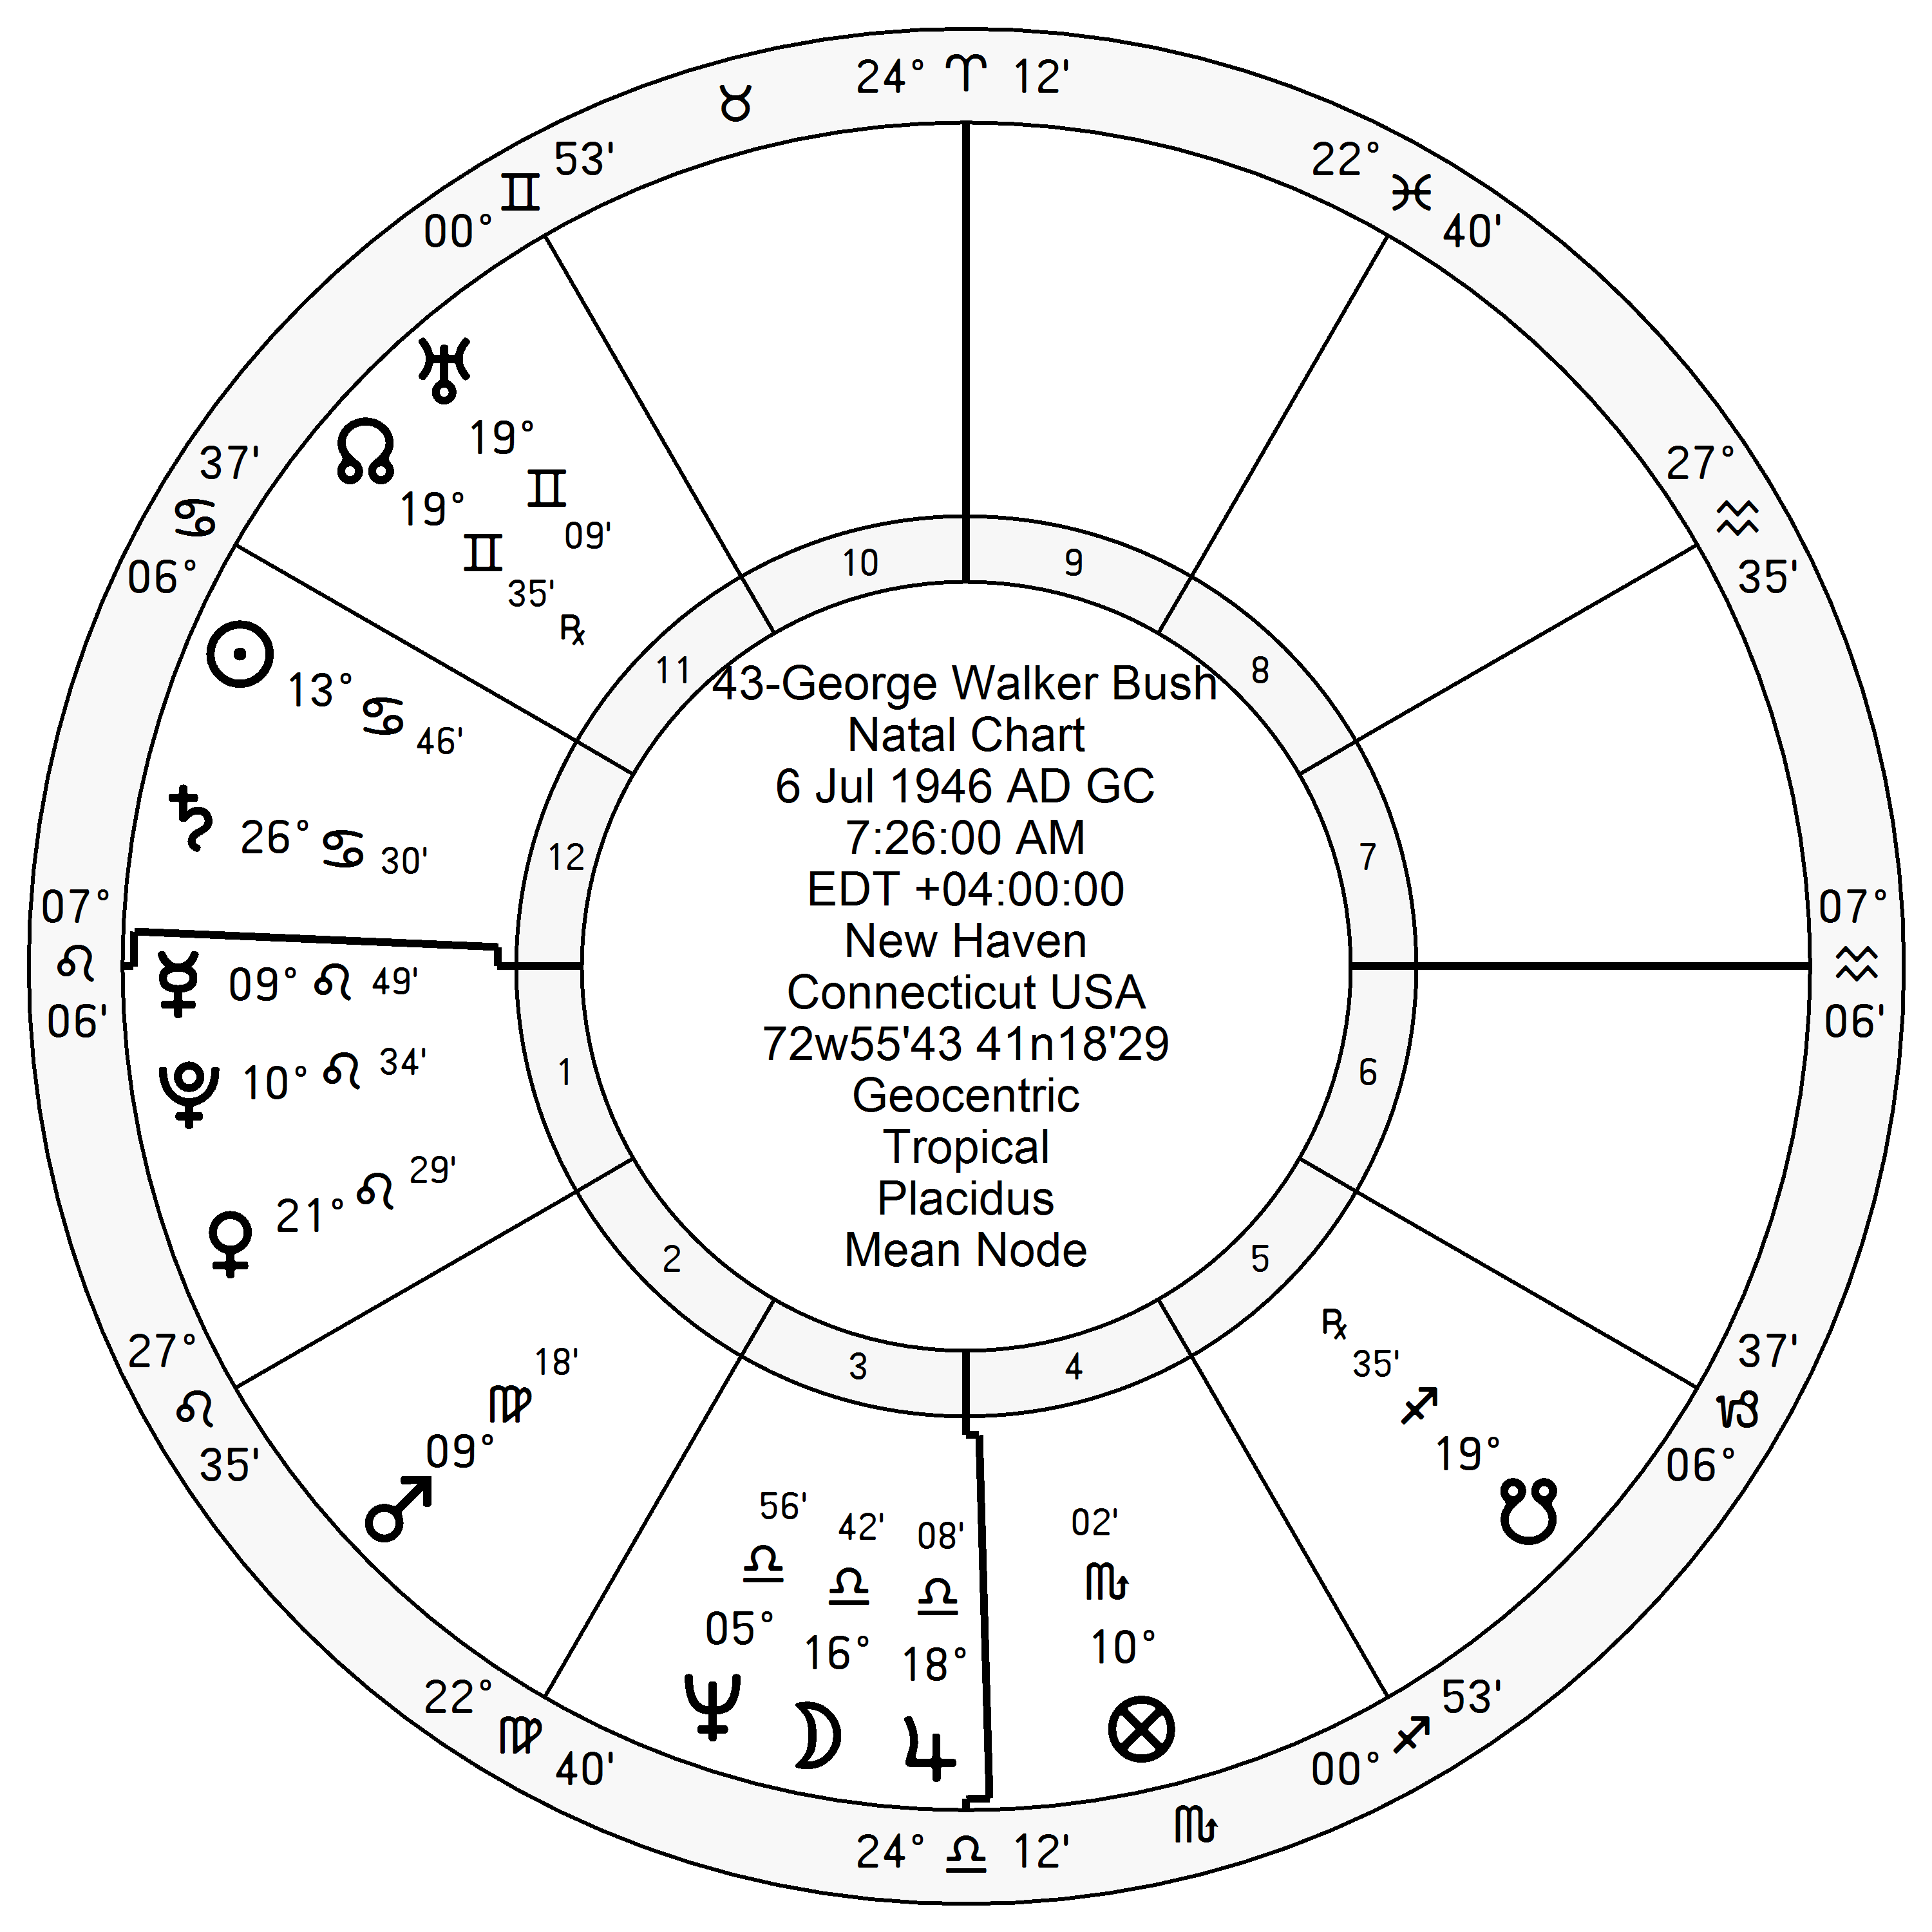
\includegraphics[width=0.9\textwidth]{charts/GW-Bush.png}}
\fontsize{7pt}{8pt}\selectfont

\Saturn\, \Trine\, P10; \Square\, N10 \\
\Mars\, \Sextile\, P10; \Trine\, N10 \\
\Mercury\, in N1 \Square\, N10, P10

\column{0.48\textwidth}
\vspace{-1em}
{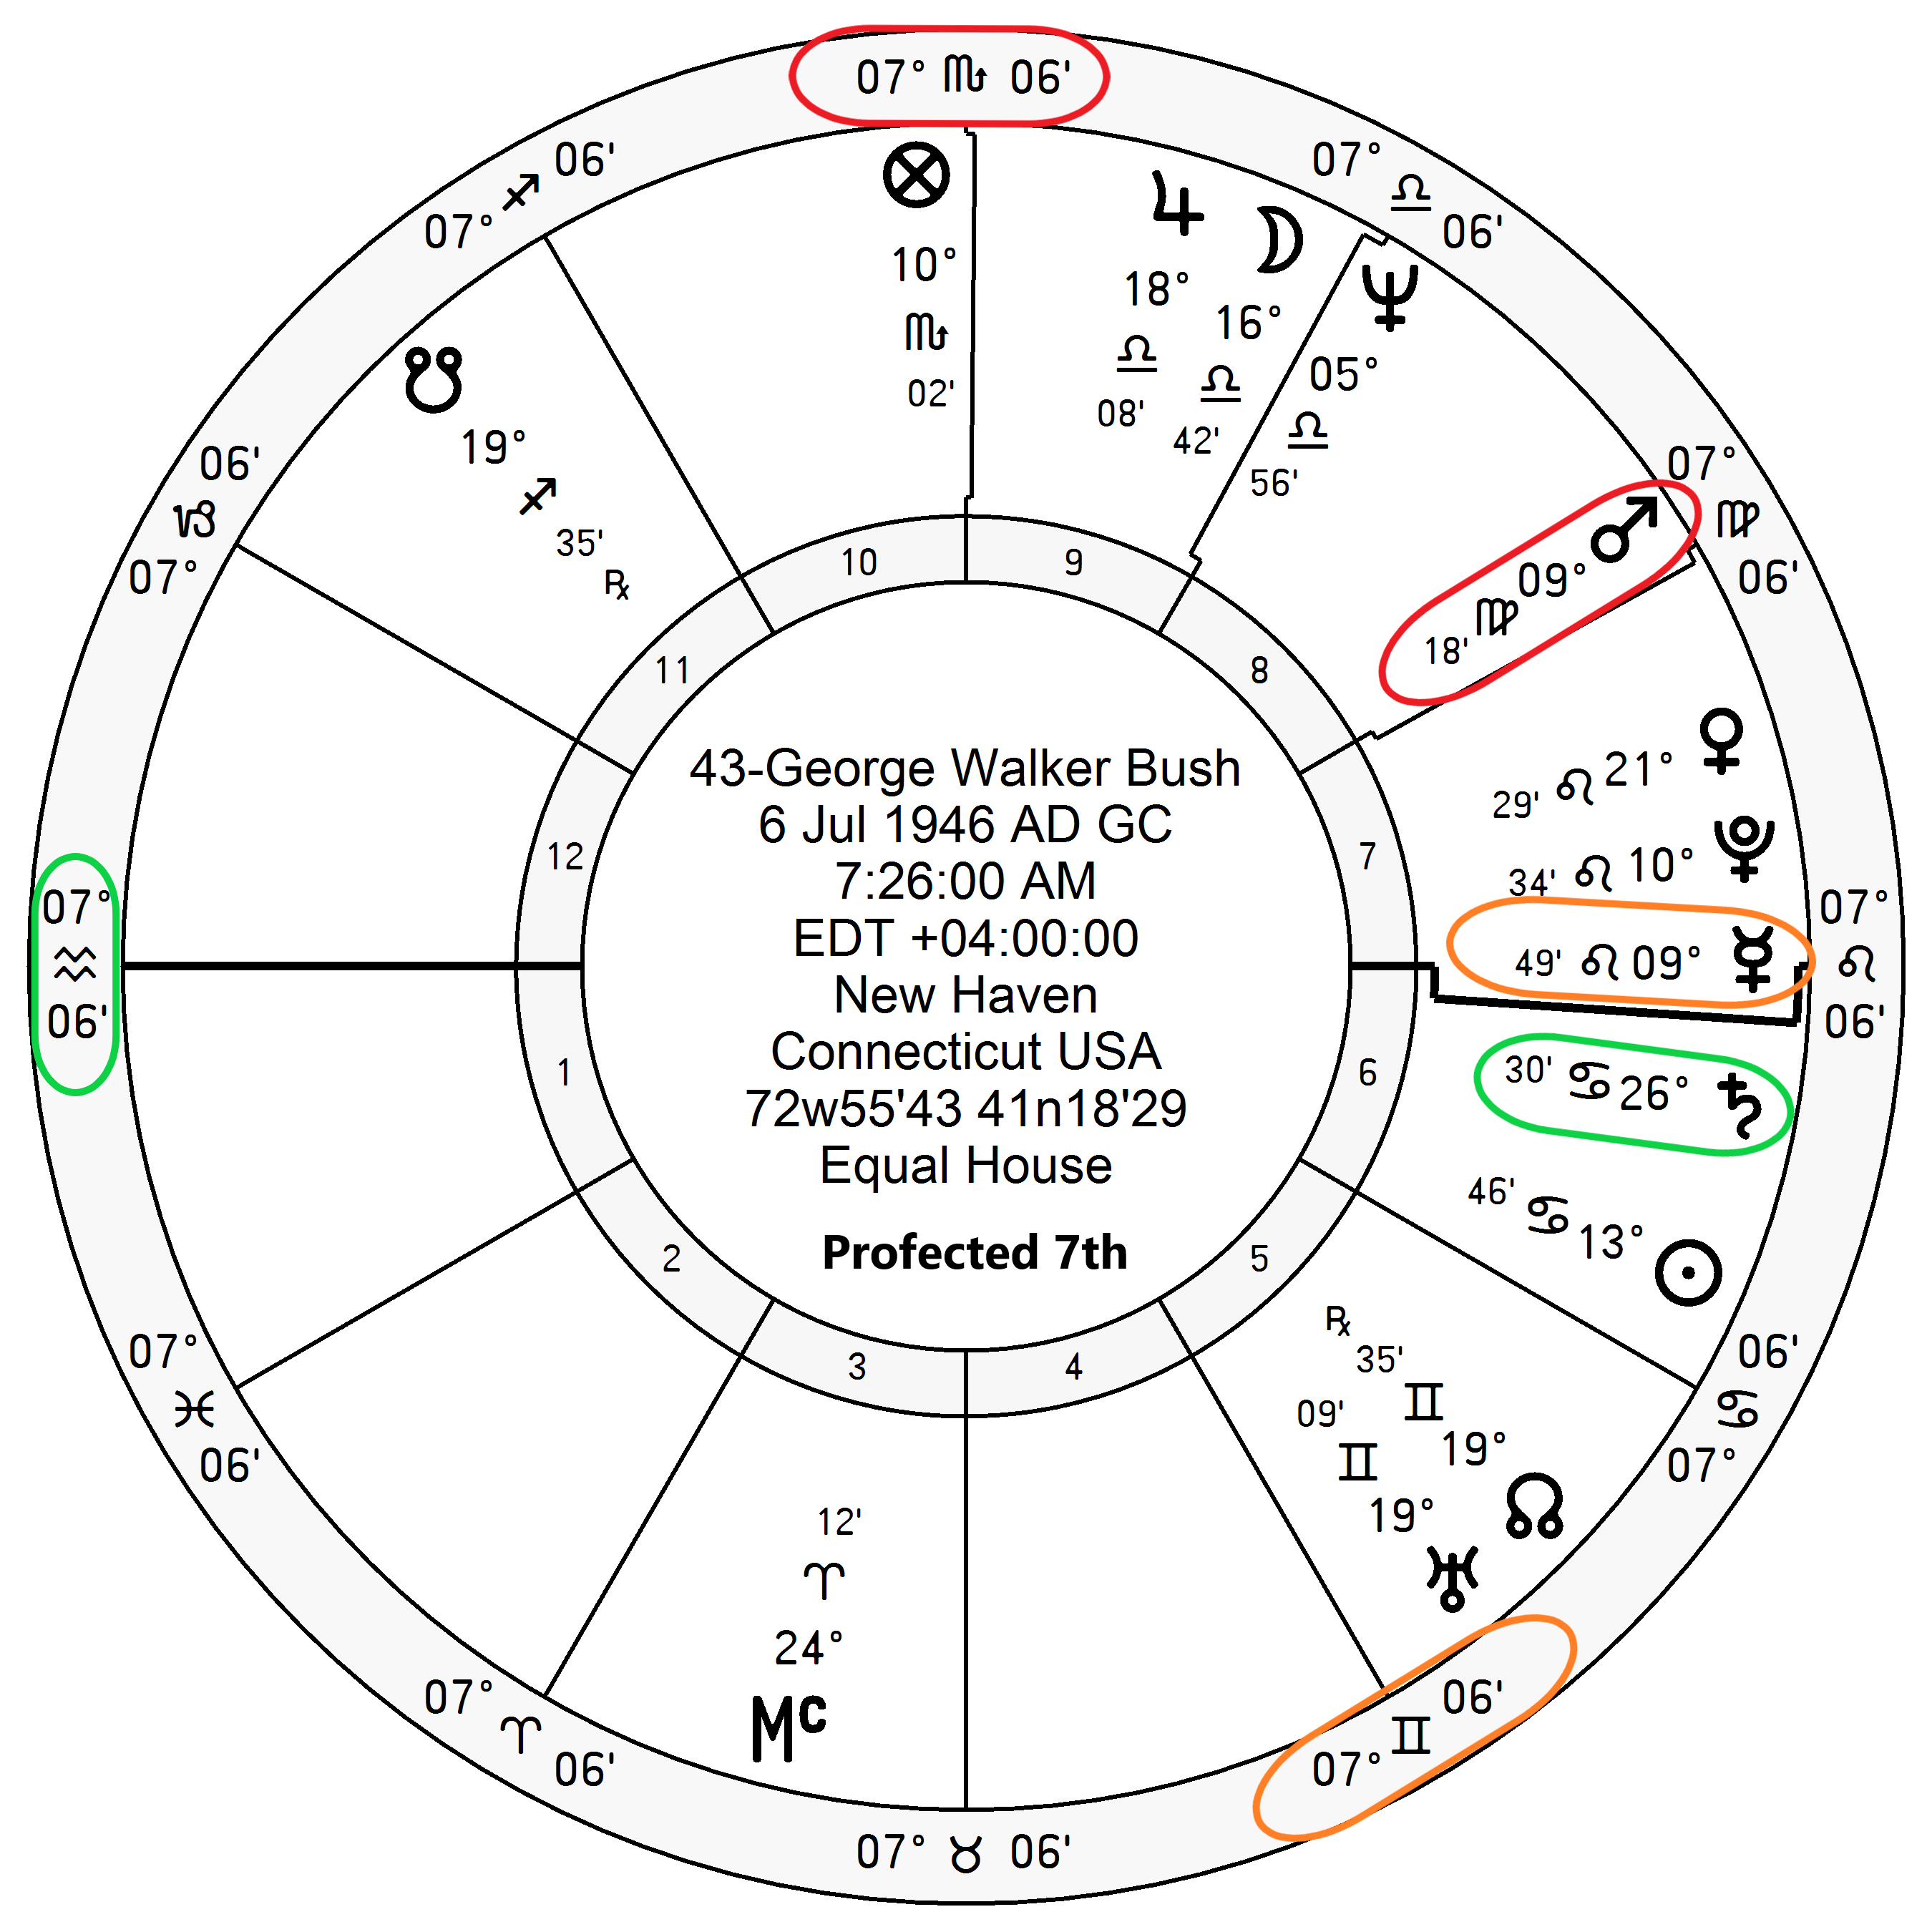
\includegraphics[width=0.9\textwidth]{charts/GW-Bush-Prof-7th.png}}
\fontsize{8pt}{9pt}\selectfont

\textbf{\dgreen P1=N7}
	$\Rightarrow$ \Saturn\, $\Rightarrow$ P6/N12\\
\textbf{\red P10}=N4
	$\Rightarrow$ \Mars\, $\Rightarrow$ P8/N2\\
PE=P5/N11
	 $\Rightarrow$ \Mercury\, $\Rightarrow$ \textbf{\dgreen P7/N1}

\end{columns}
\end{frame}

% ===================================================
\begin{frame}[t]{Election November 7, 2000: Al Gore}
\small
\begin{columns}[T, onlytextwidth]
\column{0.48\textwidth}
\vspace{-1em}
{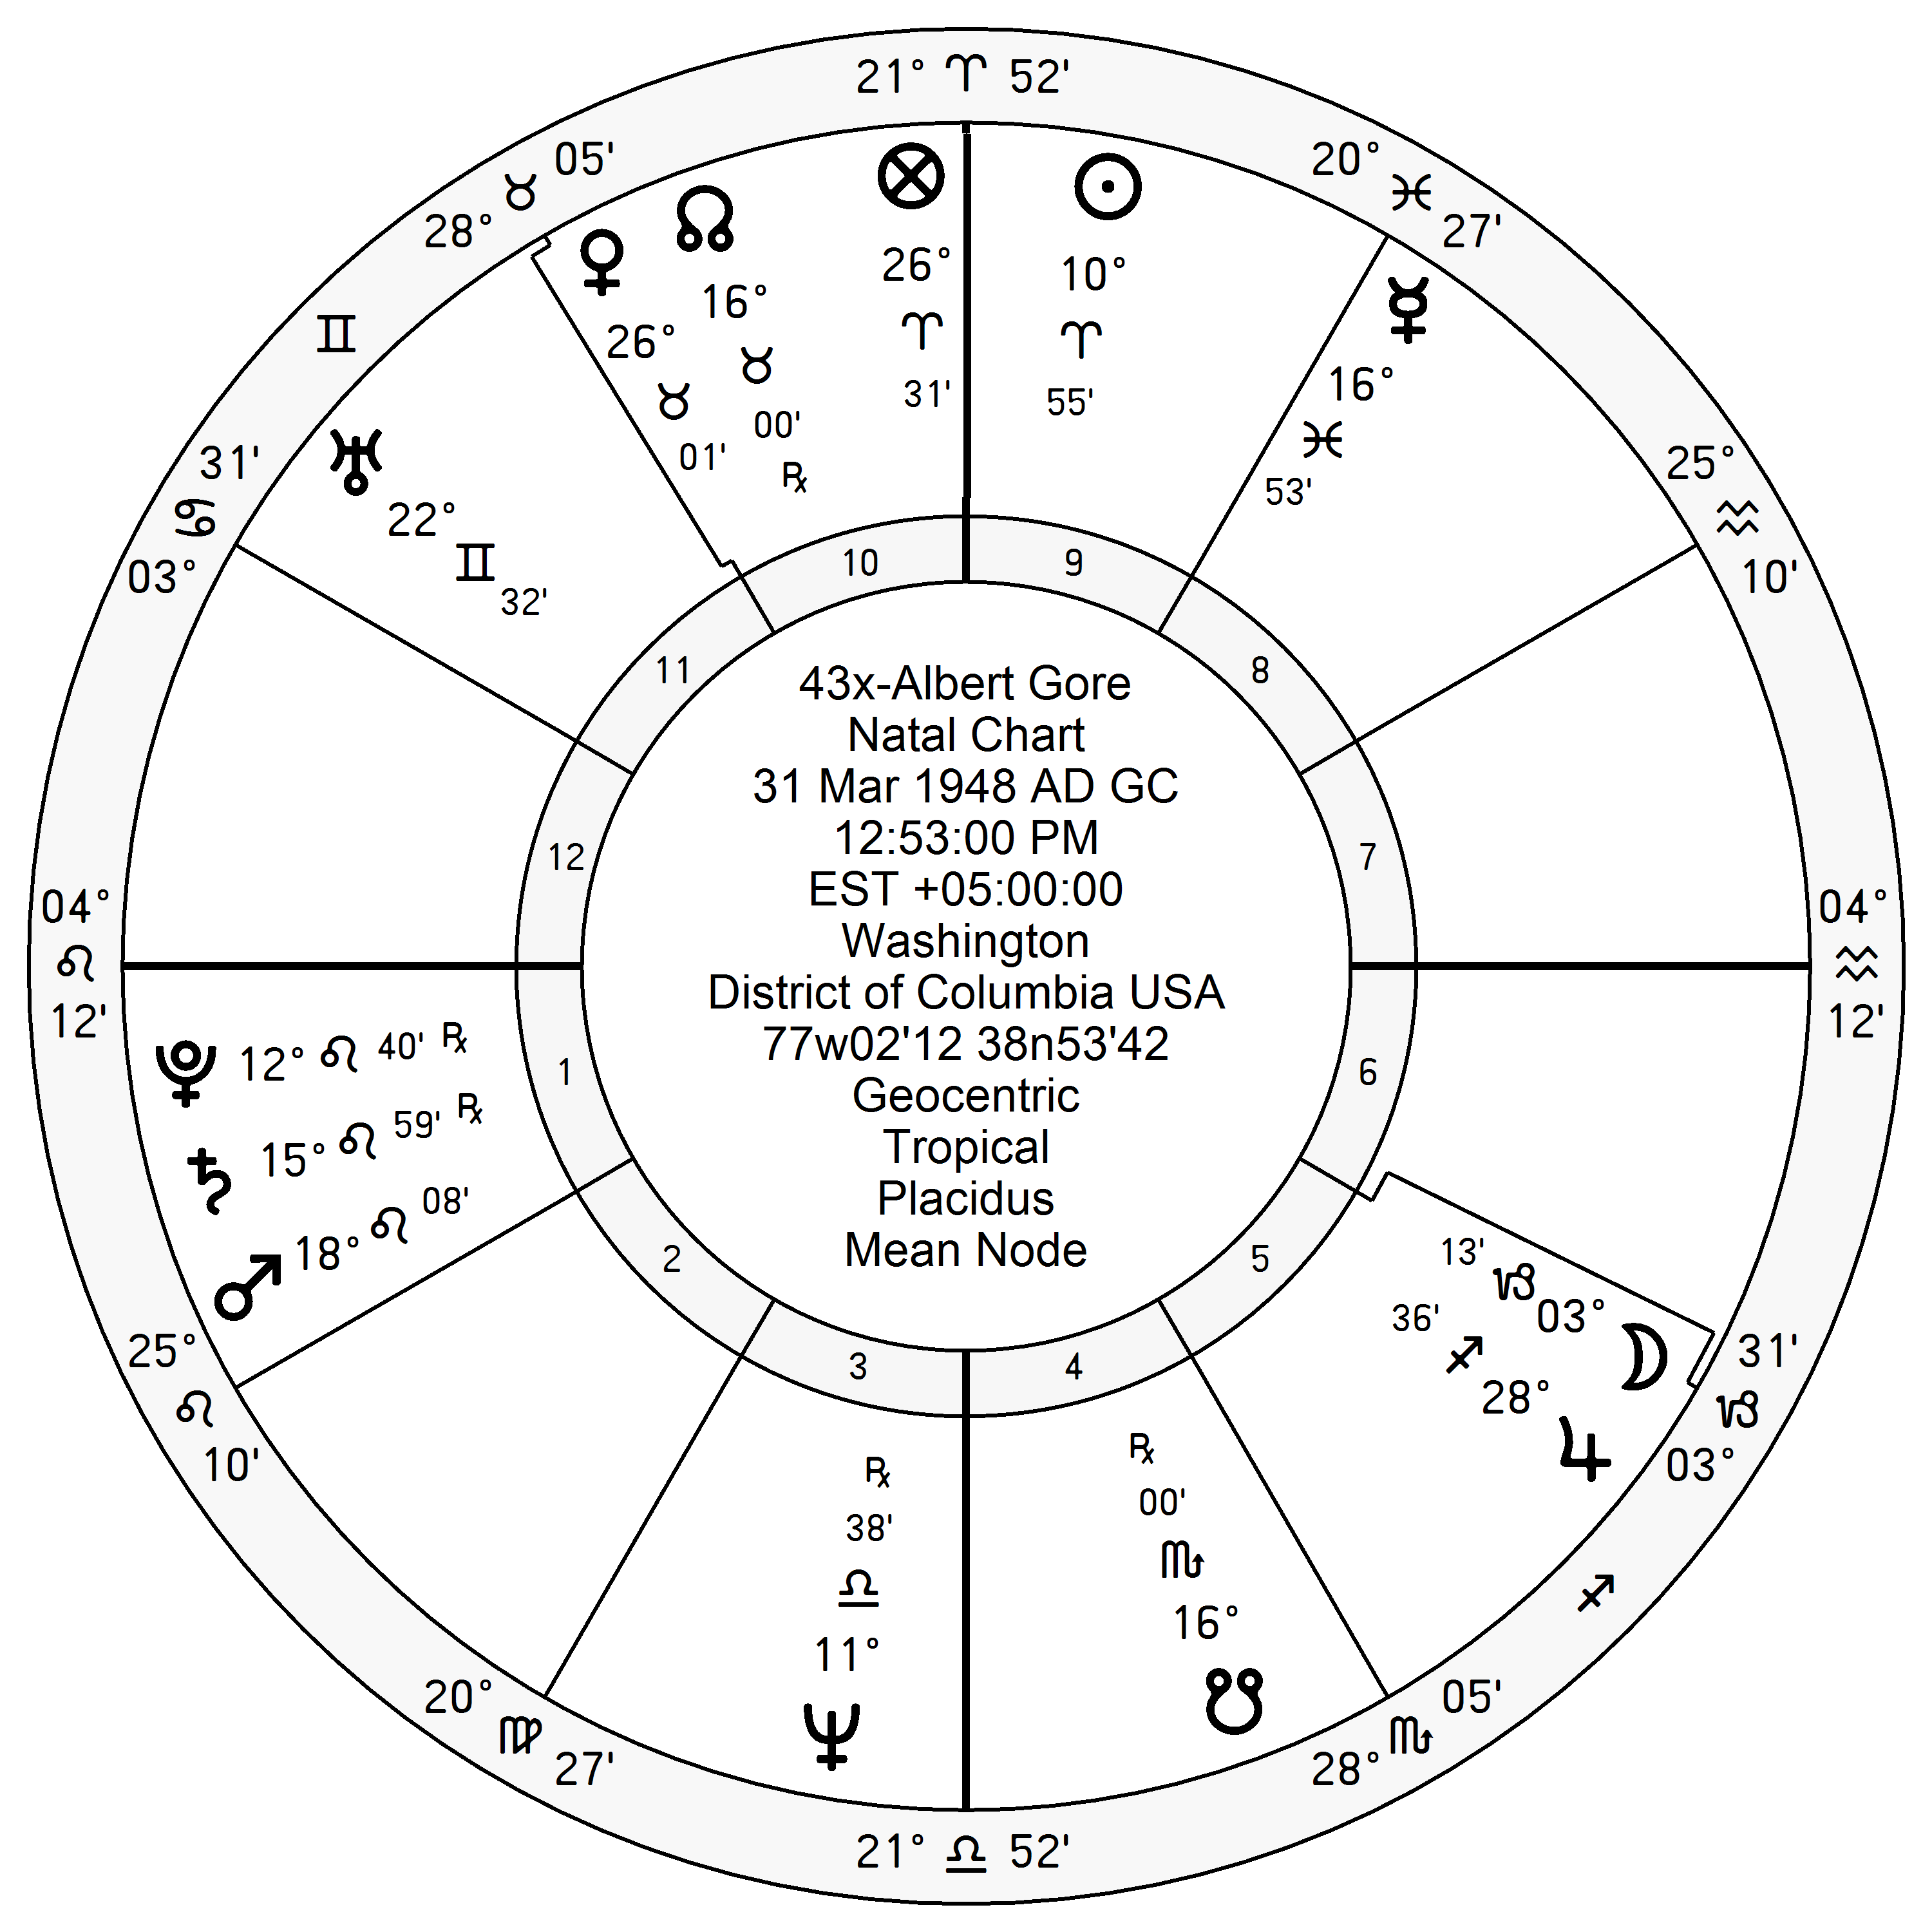
\includegraphics[width=0.9\textwidth]{charts/Gore.png}}
\fontsize{8pt}{9pt}\selectfont

\Jupiter\, in \Sagittarius\, in P1 \Square\, P10; \Trine\, N10, \Trine\, N1 \\
\Mercury\, \Opposition\, P10, \Square\, P1 \\
\Moon\, in \Capricorn\, in P1; \Square\, N10 \\
\vspace{0.5em}
There is not much between the two; Bush's radix connections to N10 are stronger.

\column{0.48\textwidth}
\vspace{-1em}
{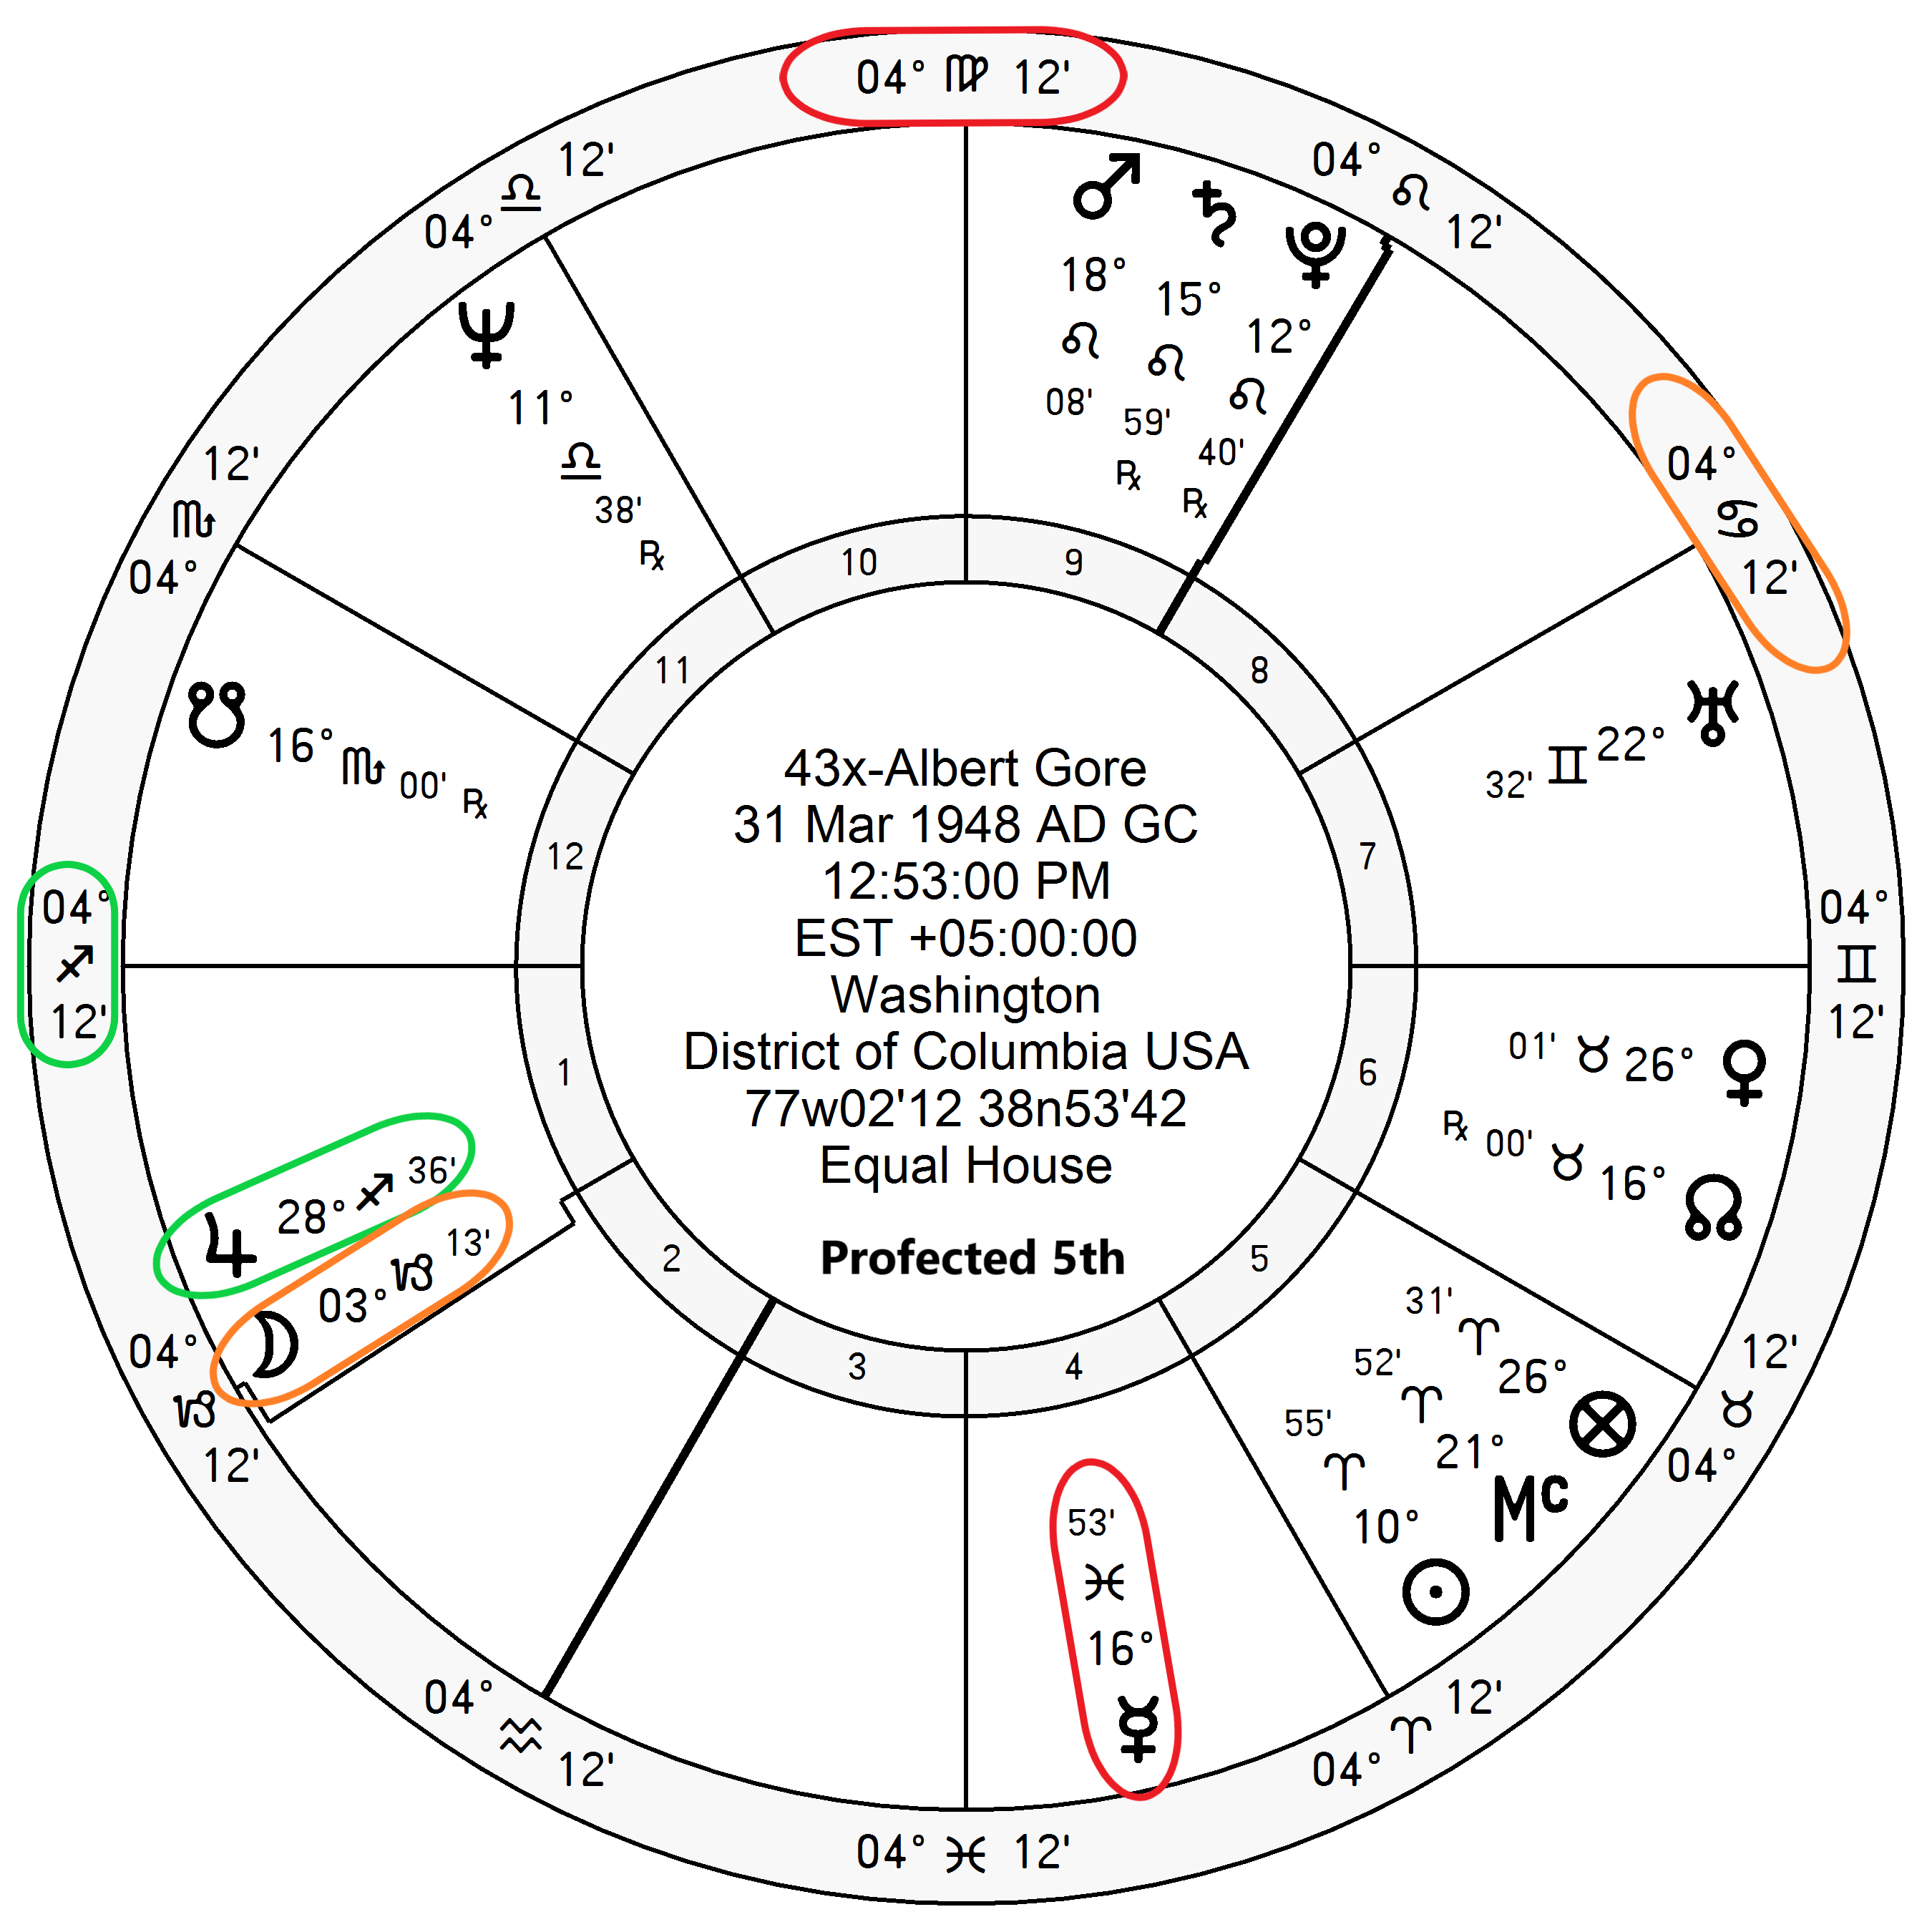
\includegraphics[width=0.9\textwidth]{charts/Gore-Prof-5th.png}}
\fontsize{8pt}{9pt}\selectfont
\textbf{\dgreen P1=N5}
	$\Rightarrow$ \Jupiter\, $\Rightarrow$ \textbf{\dgreen P1/N5}\\
\textbf{\red P10}=N3
	$\Rightarrow$ \Mercury\, $\Rightarrow$ P4/\textbf{\red N8}\\
PE=\textbf{\red P8}/N12
	 $\Rightarrow$ \Moon\, $\Rightarrow$ \textbf{\dgreen P1/N5}

\end{columns}
\end{frame}
